\section{Introduction}

%  PARAGRAPH DISEASES IN GENERAL
Coral diseases are a major threat to coral reef ecosystems and have led to significant declines in coral cover especially within the Caribbean region \citep{richardson1998coral, sutherland2004disease, aronson2001white, harvell2007coral, brandt2009dynamics}. One of the latest and the most damaging outbreaks to date in Florida's Coral Reef (FCR) is the stony coral tissue loss disease (SCTLD) \citep{noaa2018}. First observed off the coasts of Miami in 2014 by \cite{precht2016unprecedented}, the disease has since spread through the entire FCR \citep{muller2020spatial,dobbelaere2022connecting} and has been observed in several territories of the Caribbean \citep{kramer2019map, meiling2021variable, estrada2021effects,heres2021ecological}. Although the causative agent of the disease remains unknown, the hydrodynamics is likely to play an important role in its propagation as both modeling studies and ex situ experiments showed evidence of waterborne disease transmission \citep{aeby2019pathogenesis,dobbelaere2020coupled,eaton2021measuring, meiling2021variable}. Furthermore, recent studies showed that sediments can act as  a vector for the SCTLD \citep{rosales2020rhodobacterales, studivan2022reef}.

% POM
Some of the first signs of SCTLD were reported on September 26th, 2014, near Virginia Key by \cite{precht2016unprecedented}. In this study, a relationship was derived between the time of the first outbreak at the monitored reefs and their geographic distance to Virginia Key. It was therefore hypothesized that the epidemic started near Virginia Key and then spread to the neighboring reefs, both north and south. However, earlier signs of diseases were already reported north of Virginia Key in June 2014, at the monitoring site of N. Sunny Isles \citep{precht2016unprecedented}. All these observations occurred during the deepening of the Port of Miami (PoM) shipping channel, that took place between November 20, 2013 and March 16, 2015. The dredging was monitored twice-weekly at 26 permanent monitoring stations established within the Miami-Dade County, making it one of the most complete datasets related to a dredging project \citep{gintert2019regional}. Interestingly, disease signs were also reported at one of these monitoring stations in May 2014 (see supplementary material \ref{onset:appendice}).

While operating in a conventional way, dredged materials were pumped from the dredge to a spider barge and then transported to the US Environmental Protection Agency designated Ocean Dredge Material Disposal Site (ODMDS) located $\sim$8.7 km offshore. However, the suction mechanism was turned off during non-conventional rock-chopping activities in order to pre-treat very hard rock contained in the Anastasia and Fort Thompson formations between December 2013 and May 2014 \citep{miller2016detecting}. \cite{usace2017} provided a back-of-the-envelope estimation that this practice could have resulted in up to 33 cm deposition over 874,121 m$^2$ of reef surrounding the outer entrance channel . Additionally, several studies reported that the impact of the dredging was widespread \citep{miller2016detecting}, causing the death of  $> 560,000$ corals within 0.5 km of the channel \citep{cunning2019extensive} and producing sediment plumes covering up to 11 km$^2$ of coral area within 5-10 km of the dredging operations \citep{barnes2015sediment}.

% SEDIMENTS
Sediments released by dredging can affect the biological functions of corals in numerous ways  through turbidity and sedimentation \citep{erftemeijer2012environmental,jones2015effects}. Increased turbidity caused by the suspended sediments reduces the light available to symbiotic zooxanthellae, leading to reduced coral cover and growth. Sedimentation, on the other hand, can cause smothering or burial of coral polyps \citep{erftemeijer2012environmental,jones2015effects,jones2019sediment}. Furthermore, both sedimentation and turbidity can significantly reduce larval recruitment by inhibiting settlement and reducing larval survival in the water column \citep{jones2015effects}. These effects are stronger with fine-grained sediments, as they cause a stronger light reduction \citep{storlazzi2015influence,fourney2017additive}. Additionally, fine-grained sediments such as silts have high nutrient contents, which can lead to an increased microbial activity, eventually causing anoxic conditions in the immediate vicinity of corals \citep{weber2012mechanisms}. As they release finer sediments over significantly longer periods than natural events such as hurricanes, dredging activities can thus be more harmful to corals and reef habitat compared to other types of sedimentation \citep{cunning2019extensive}.

% ON ENTRE DANS LE VIF DU SUJET
Nonetheless, \cite{gintert2019regional} argued that the reported coral mortality during the dredging project was dominated by the regional outbreak of SCTLD. Further, they suggested that the onset of the disease might have been linked to a leaking discharge pipe of the Miami Central District Municipal Wastewater Treatment Plant (WWTP) located off Virginia Key. However, as sediments can act as vector for SCTLD \citep{studivan2022reef}, there is also a possibility that the causative agents of the disease were transported to the monitoring site of Virginia Key by sediments released during the dredging. This scenario can be evaluated using a sediment transport model. As coastal reef ecosystems are characterized by the complex topography of the coastline and the presence of islands, reefs and artificial structures, such a model would require a fine spatial resolution to accurately represent the transport of sediments at the reef-scale. In this context, unstructured-mesh models are particularly well suited, as they can easily adapt to the topography \citep{fringer2019future} and can capture small-scale circulation features around reefs and islands \citep{lambrechts2008multi}.

The goal of this study is therefore to simulate the dispersed sediments during the entirety of the PortMiami Deep Dredge Project (PMDDP) using a high-resolution hydrodynamic model coupled with a sediment transport model. Specifically, our goal is to answer the following questions: (1) Which reefs were impacted by the PMDDP and was this impact consistent with the observed timing of the onset of SCTLD ?  (2) Was disease transmission to Virginia Key from other diseased reefs possible before September 2014 ? 

% === METHODS === %
\section{Methods}

\begin{figure}
	\centering
	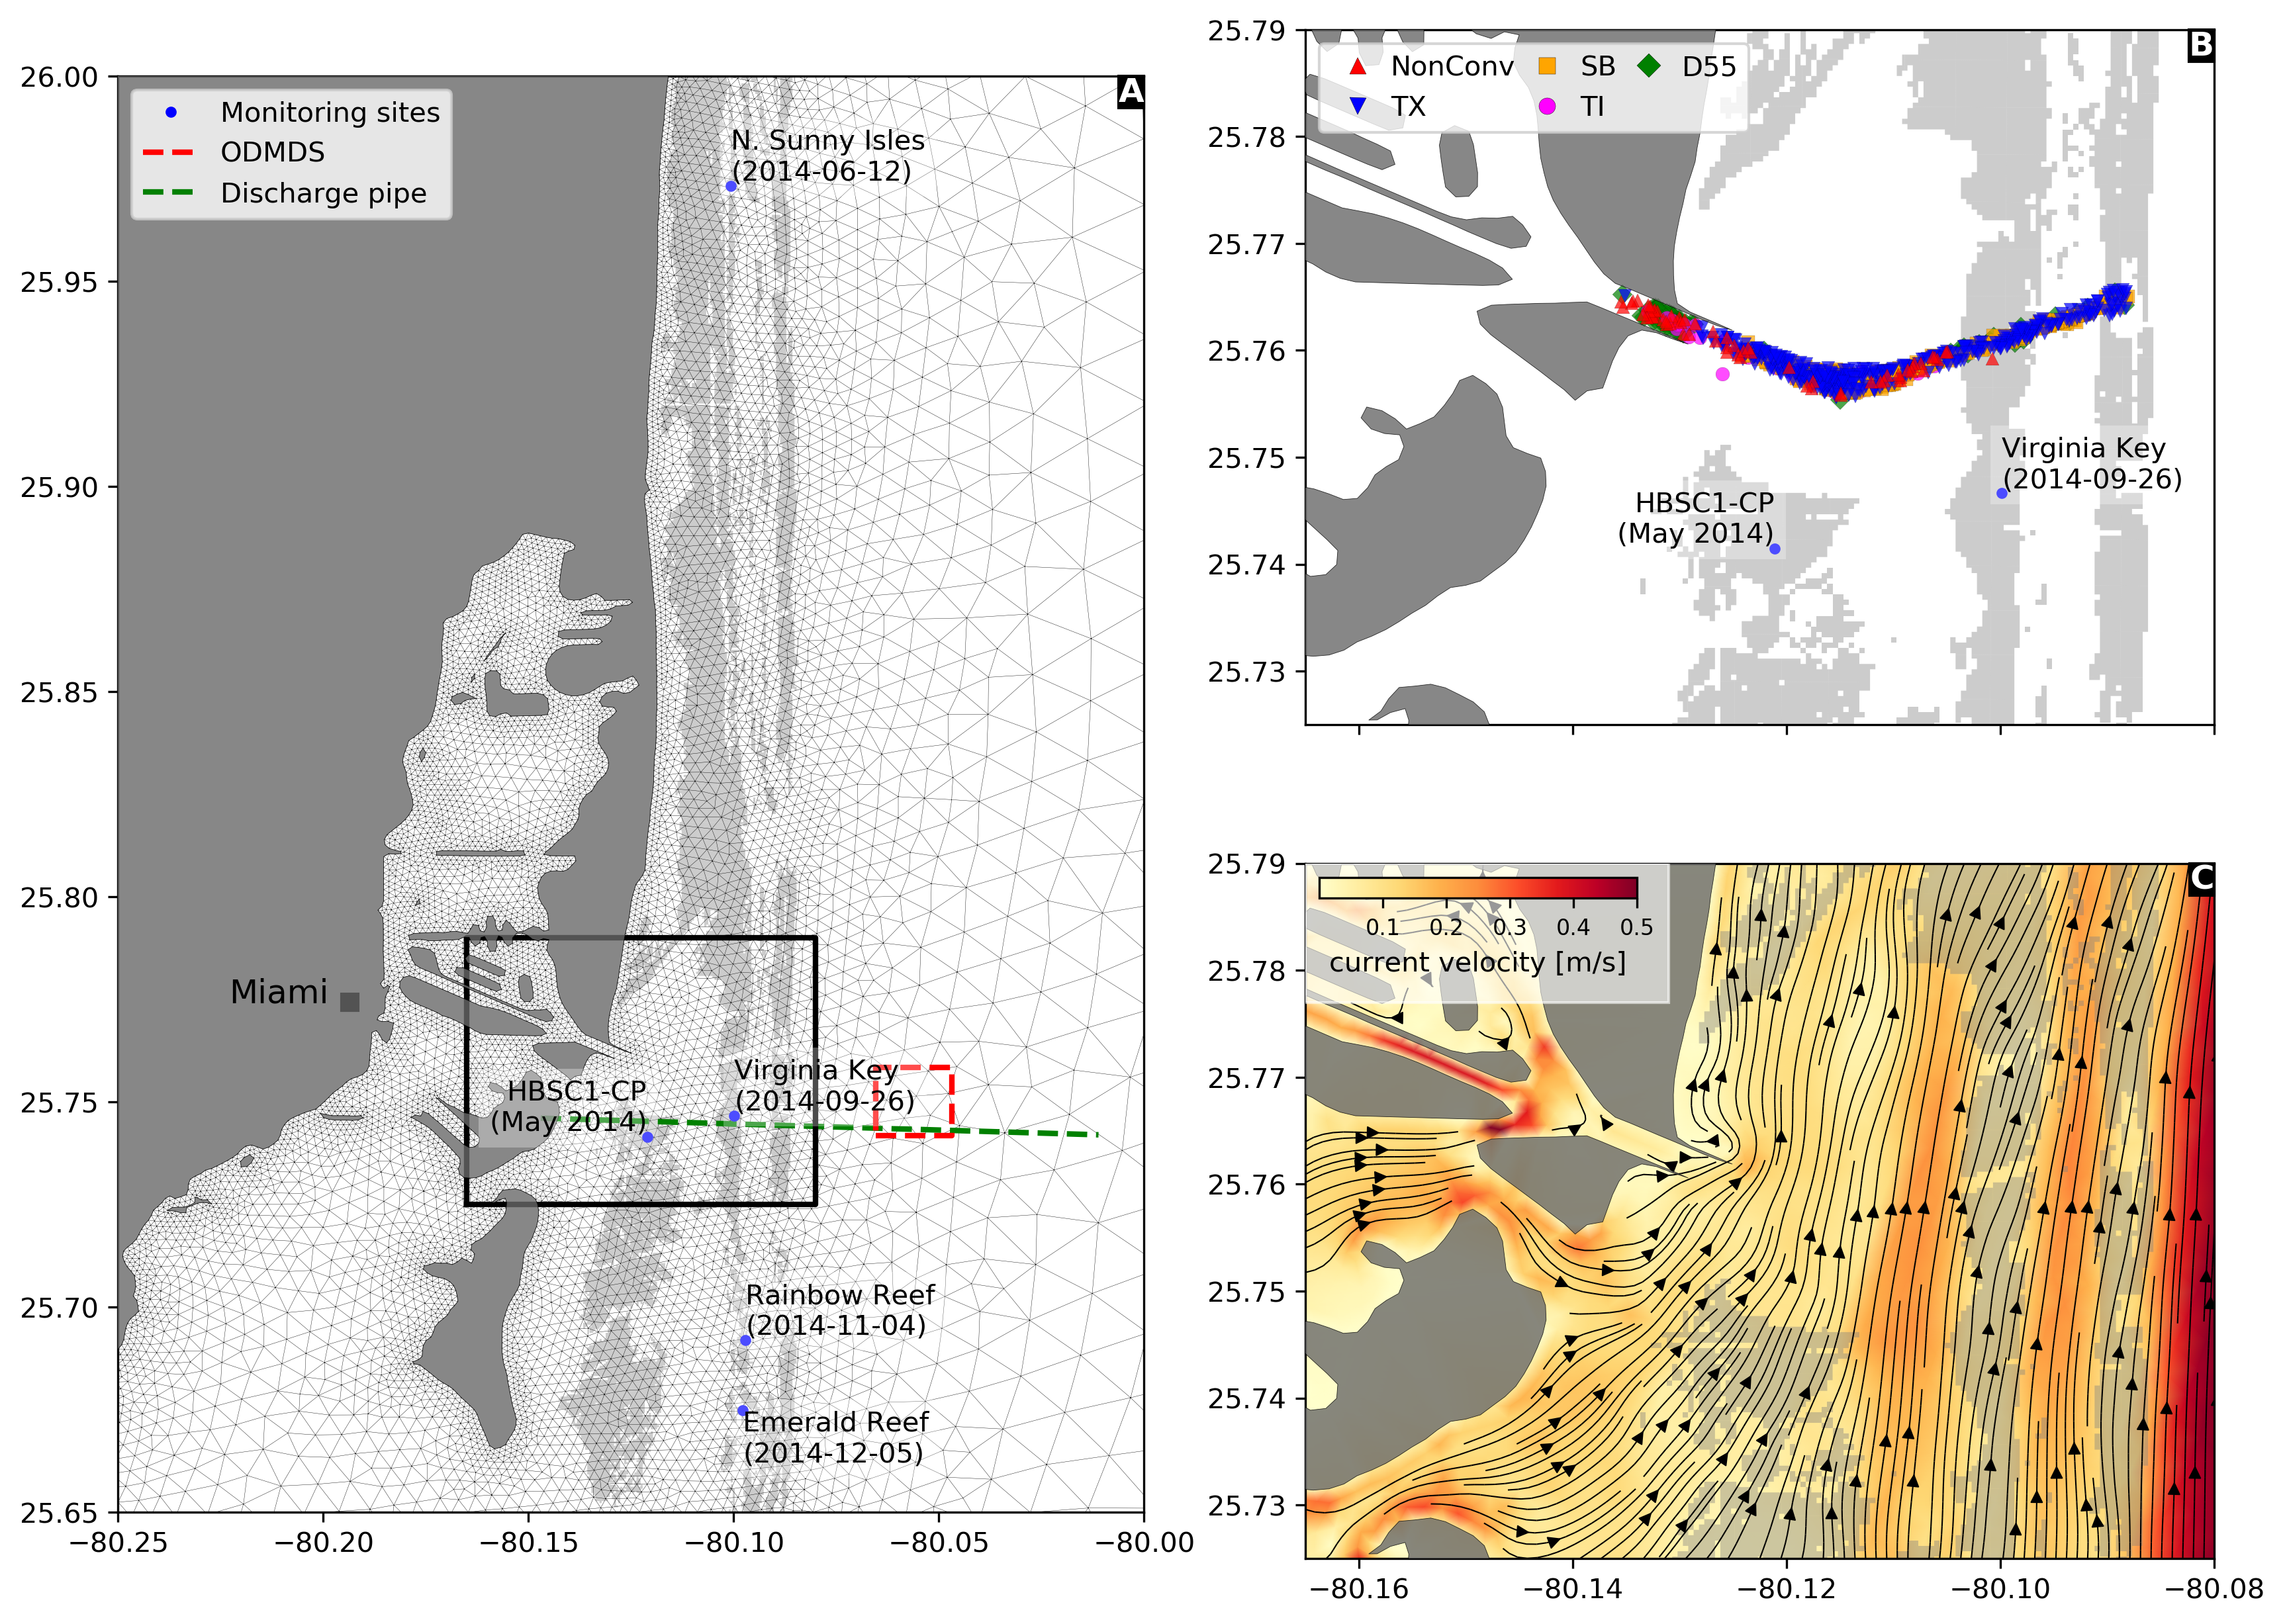
\includegraphics[width=\textwidth]{chapters/onset/figures/fig_mesh_onset.png}
	\caption{\textbf{A}: Model mesh near the dredged channel. Elements have a characteristic length of 100 m over reefs (in light grey) and along the coasts (in dark gray). The monitoring sites considered in the present study are shown by blue dots. The date of the first reported signs of SCTLD at these sites is given between brackets. The Ocean Dredge Material Disposal Site (ODMDS) is shown in red and the discharge pipe of the Miami Central District Municipal Wastewater Treatment Plant in green. \textbf{B}: Close up view of the dredged channel. The locations of the different types of dredging that took place during the expansion of PoM are shown by colored markers. \textbf{C:} Snapshot of the modeled currents in the vicinity of the dredged channel. Small-scale flow features such as the acceleration of currents between reefs and islands are well reproduced by the model.}
	\label{fig:onset_mesh}
\end{figure}

The hydrodynamics of the entire FCR was modeled using the multi-scale ocean model SLIM\footnote{\url{ https://www.slim-ocean.be}}, which has already been extensively validated in the area \citep{frys2020fine,dobbelaere2020coupled,dobbelaere2022impacts,dobbelaere2022connecting}. SLIM uses an unstructured mesh whose resolution can be locally increased in order to accurately represent fine-scale flow features. The mesh used in this study was built following the same methodology as \cite{dobbelaere2020coupled}, with a local refinement near PoM and in the Bay of Biscayne to achieve a resolution of 100 m in the vicinity of the dredged channel (Fig. \ref{fig:onset_mesh}A). It was made up of approximately $3.5\times 10^5$ triangles and was generated with the seamsh\footnote{\url{https://pypi.org/project/seamsh/}} Python library, which is based on the the open-source mesh generator GMSH \citep{geuzaine2009gmsh}. The model was run between October 15, 2013 and September 26, 2014 to cover the whole dredging period prior to the observation of SCTLD on Virginia Key by \cite{precht2016unprecedented}. Using such a fine mesh resolution, we simulated fine-scale details of the ocean currents, such as the flow acceleration between reefs and islands (Fig. \ref{fig:onset_mesh}C).

The transport of sediments released from dredging operations along the channel was then modeled using a Lagrangian particle tracking model, forced by the simulated currents. The sediment model is inspired by the Particle Transport Model (PTM), developed by the US Army Corps of Engineers \citep{macdonald2006ptm}. In this model, particles undergo a combination of horizontal and vertical motions. The vertical dynamics is mostly driven by gravity, with heavier particles sinking faster. Once they have settled, particles can be resuspended when shear stress exceeds   the critical Schields parameter, as parameterized by \cite{soulsby1997threshold}. The horizontal motion of the suspended particles is derived from the 2D model velocity by assuming a vertical log profile, hence yielding a quasi-3D approach. When sediment particles enter the near-bed zone, their horizontal velocity is greatly reduced and sediments are transported with the bedload.   

As sediment dispersion is dependent on the grain size, we modeled the dispersal of five sediment classes to represent impacts of fine- to coarse-grained particles: (\textit{i}) 5-50 $\mu$m, (\textit{ii}) 50-100 $\mu$m, (\textit{iii}) 100-200 $\mu$m, (\textit{iv}) 200-300 $\mu$m, and (\textit{v}) 300-400 $\mu$m. We performed a  different simulation for each class, with the grain size randomly drawn from a uniform distribution over the corresponding size range. The density of each sediment particle was derived from its size using the formula of \cite{hamilton1982sound}. Furthermore, all particles were differentiated based on the type of dredge that produced them. Five types of dredge were considered in our modeling study (Fig. \ref{fig:onset_mesh}B): (\textit{a}) Texas cutterhead (TX), (\textit{b}) non-conventional dredging, \ie~TX with suction mechanism turned off (NonConv), (\textit{c}) Spider Barge (SB), (\textit{d}) Terrapin Island hopper (TI), and (\textit{e}) Dredge 55 clamshell (D55).

Dredging operations performed during the expansion of PoM were characterized in our dataset by a date, a location and  a type of dredge (Fig. \ref{fig:onset_mesh}B). In the absence of information about the exact time of the dredging, sediment particles were released from the dredging location during a whole day at a rate of 80 particles/hour in the model. To account for the motion of spider barges between the dredging and disposal sites, particles were released every 500 m along a straight line joining the dredging location to the ODMDS (see Fig. \ref{fig:onset_mesh}A) for every dredging operation labelled as SB.

The outputs of the sediment model were then used to evaluate the turbidity and sedimentation generated by the different dredging operations over coral reefs. The occurrence of high turbidity over reefs was assessed based on the concentration of suspended sediment particles in the model. This concentration was computed by counting the number of suspended particles inside the cells of a regular 200 m $\times$ 200 m grid over our computational domain. The modeled occurrence of plume was then compared against daily data of plume detection. This dataset was derived from satellite imagery by \cite{cunning2019extensive}\footnote{datasets available at \url{https://github.com/jrcunning/pom-dredge/}} following the methods of \cite{barnes2015sediment} at sites located within 15 km of the dredged channel. As in these two previous studies, we computed  the simulated plume frequency by dividing the number of days during which plumes occurred by the total number of simulated days for all grid cells. The impact of sedimentation was quantified by computing the cumulated concentration of settled particles within the same computational grid. This cumulated concentration was normalized by the total number of simulated time steps to obtain an averaged concentration of deposited particles over the simulated period. Higher values of this indicator would indicate larger sediment deposition over a longer cumulated time.

The potential impact of dredging on the onset of the SLD outbreak was more specifically assessed at five monitoring sites were signs of disease were reported. Four sites were reefs where disease was reported in 2014 by \cite{precht2016unprecedented}. The fifth site was the monitoring station HBSC1-CP, used throughout the expansion of PoM, where signs of disease were already reported in May 2014 (Fig. \ref{fig:onset_mesh}A, see supplementary material \ref{onset:appendice}). The impact of dredging was assessed by counting the total number of sediment particles originating from each dredging that were transported within 500 m of all five site. This distance was chosen to match the scale of the 500 m $\times$ 500 m reef polygons used in the model \citep{dobbelaere2020coupled}. The resulting numbers of particles were then divided by the total number of sediment particles released by each type of dredging operation. Larger values of this indicator would suggest a greater impact of a given type of dredging operation at a given monitoring sites.  

Finally, as previous studies showed evidence of waterborne transmission of SCTLD \citep{aeby2019pathogenesis, dobbelaere2020coupled,eaton2021measuring, meiling2021variable}, there is a possibility that the disease propagated to Virginia Key from other diseased reefs affected prior to September 2014. To evaluate this possibility, we computed monthly disease connectivity matrices following the methodology of \cite{dobbelaere2020coupled} during our simulated period. These connectivity matrices can be interpreted as large graphs whose vertices are 500 m $\times$ 500 m sub-reef polygons and whose edges represent disease connectivity pathways. Evaluating the possibility of disease propagation from any sub-reef $A$ to any sub-reef $B$ is therefore equivalent to evaluating the existence of paths, \ie~sequences of connected vertices in the network starting from $A$ and reaching $B$. As computing all possible paths is not computationally tractable, we limited ourselves to the computation of shortest paths from any given reefs to the Virginia Key monitoring site. This was performed using the function \texttt{get\_all\_shortest\_paths} of the Python \texttt{python-igraph} package \citep{csardi2006igraph}. Such a function requires the definition of a weight $w_{ij}$ for the edge connecting reef $i$ to reef $j$. We chose $w_{ij} = 1-\tilde{C}_{ij}$, where $\tilde{C}_{ij}$ is the probability of disease propagation from reef $i$ to reef $j$, so that "shorter" edges of the networks (\ie~connectivity pathways with smaller weights) correspond to connections with larger disease propagation probability. The probability of a given path was then defined as the mean connection probability of the edges composing this path.

Finally, the 2D mode of the particle tracking model was used to assess the impact of wastewater leaking from the discharge pipe mentioned by \cite{gintert2019regional}. This model simulates the transport of neutrally buoyant material driven by mean current within the water column \citep{dobbelaere2020coupled}. Without clear information about the location of the leak, particles were continuously released every 100 m along a straight line between Miami Central District Municipal WWTP, located on Virginia Key and the ocean discharge outfall located at 25$^\circ$44'31''N 80$^\circ$05'10''W \citep{koopman2006ocean}. The impact of wastewater released from the different potential leak locations was then evaluated by computing the fraction of released wastewater particles that were transported within 500 m of the site of Virginia Key.

%%%%%%%%%%%%%%%%%%%
% --- RESULTS --- %
%%%%%%%%%%%%%%%%%%%
\section{Results}

Only grain sizes in the 5-50 $\mu$m range produced plumes consistent with the observations of \cite{barnes2015sediment} and \cite{cunning2019extensive} (Fig. \ref{fig:onset_depo}A). For larger grain sizes, particles settled in the direct vicinity of the channel. For these heavier particles, suspended sediments were only observed offshore, closer to the Florida Current, where the current velocity was sufficiently strong to prevent deposition. This suggests that the observed turbidity was mostly due to fine silts. The modeled occurrence of plumes within 15 km of the dredged matched the presence/absence data of \cite{cunning2019extensive} in 82.7\% of cases and the total area where plumes were observed was about 230 km$^2$, consistent with the $\sim$228 km$^2$ estimated by \cite{barnes2015sediment}. Modeled plumes mostly occurred north of the dredged channel, as particles were driven northward under the action of the Florida Current, with plume occurring during 20\% of the simulated days near the monitoring site of N. Sunny Isles. Plume frequencies were lower ($\sim$5\%) over offshore reefs but reached of up to 50\% over alongshore reefs. These alongshore reefs correspond to regions of important sedimentation (Fig. \ref{fig:onset_depo}B), which is consistent with the correlation between plumes and sedimentation highlighted in \cite{cunning2019extensive}. The plume frequency was about 1\% at site of HBSC1-CP while no plume reached other southern monitoring sites during the simulation. 

% \begin{table}
	%     \centering
	%     \begin{tabular}{|l|cccc|}
		%         \hline
		%          & Threshold         & Accuracy & False positive  & False negative \\
		%          & [particles/m$^2$] & [\%]     & [\%]            & [\%]  \\
		%         \hline
		%         5-50 $\mu$m    & 21 & 86.678 & 2.912 & 10.410 \\
		%         50-100 $\mu$m  & 20 & 83.058 & 8.525 & 8.417 \\
		%         100-200 $\mu$m & 30 & 84.814 & 7.133 & 8.053 \\
		%         200-300 $\mu$m & 18 & 84.459 & 7.988 & 7.553 \\
		%         300-400 $\mu$m & 13 & 84.615 & 8.140 & 7.244 \\
		%         \hline
		%     \end{tabular}
	%     \caption{Validation of the modeled presence of plumes against plume observations from satellite imagery. Overall, the model agrees well with observations}
	%     \label{tab:onset_val} 
	% \end{table}

\begin{figure}
	\centering
	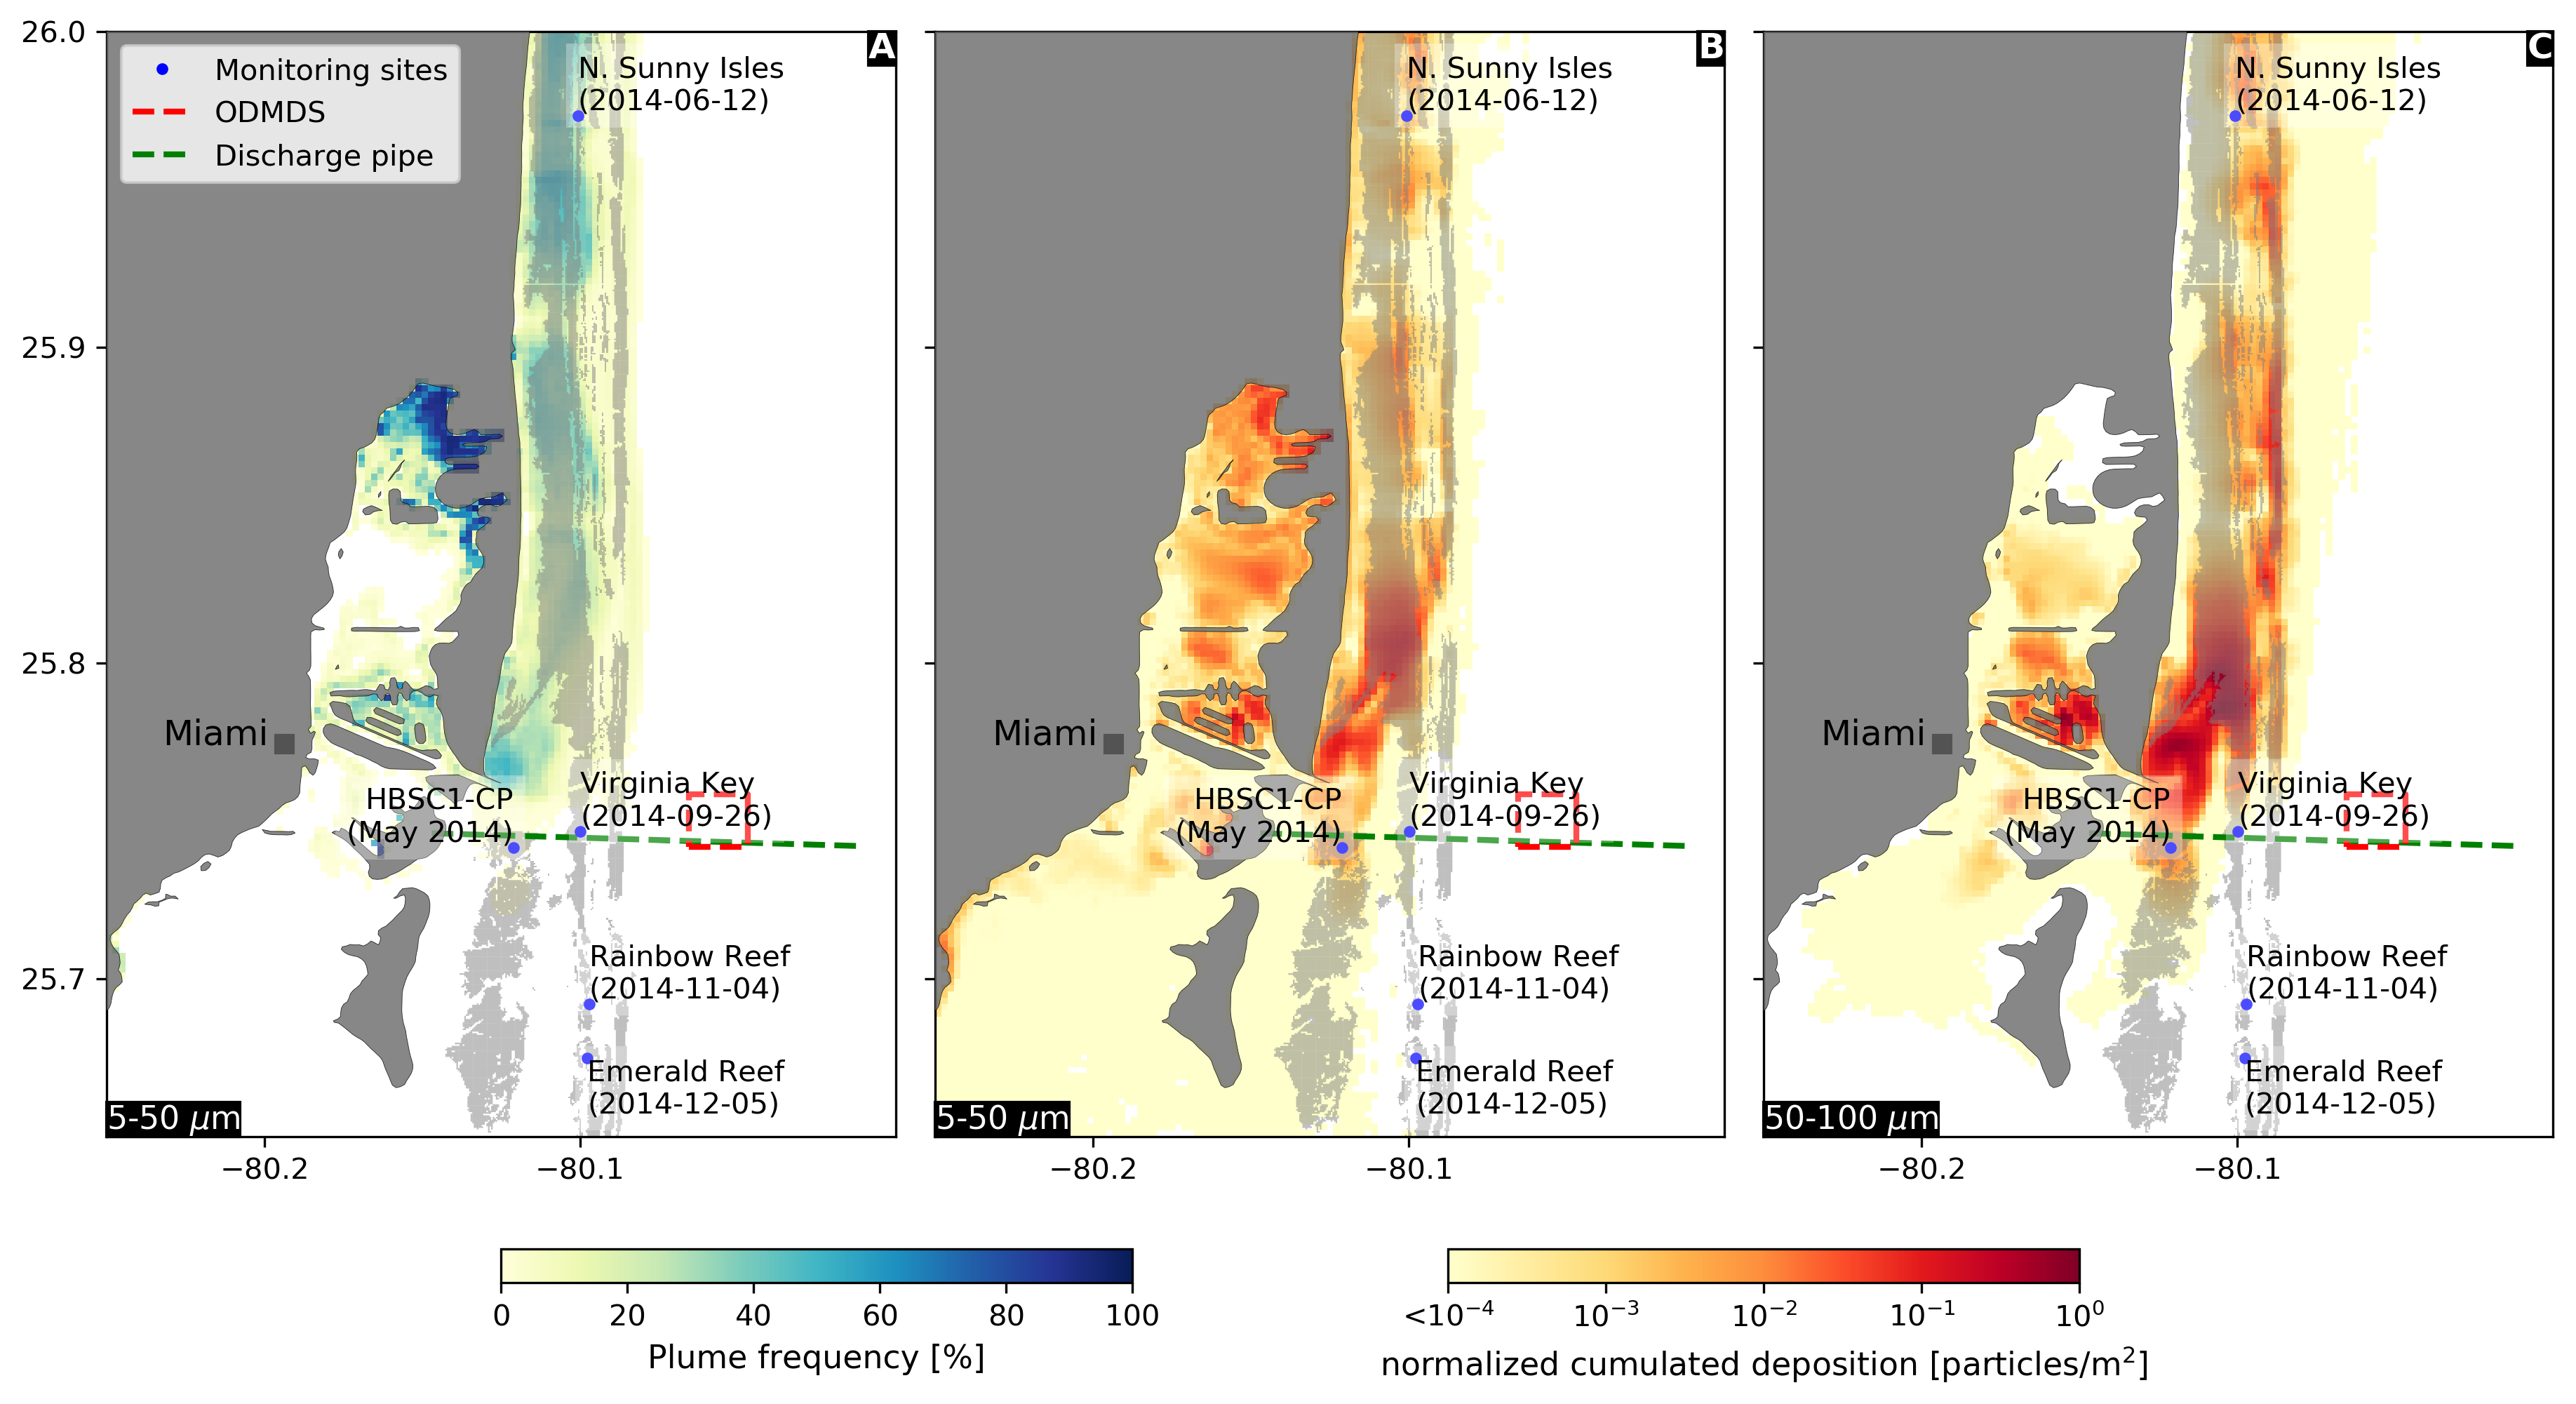
\includegraphics[width=\textwidth]{chapters/onset/figures/deposition_plumes.png}
	\caption{\textbf{A}: Plume frequency for grain size in the range 5-50 $\mu$m. The averaged concentration of deposited sediments are shown for grain sizes more likely to carry the disease: 5-50 $\mu$m (\textbf{B}) and 50-100 $\mu$m (\textbf{C}). Most modeled turbidity and sedimentation occurred north of the dredged channel. Non negligible sediment deposition occurred at site HBSC1-CP.}
	\label{fig:onset_depo}    
\end{figure}

Deposition results are shown for grain sizes corresponding to silts, which are more likely to carry organic matter and therefore more likely to carry SCTLD agents \citep{erftemeijer2012environmental}(Fig. \ref{fig:onset_depo}B,C). Sedimentation mostly occurred on reefs located north of the dredge channel. For grain sizes smaller than 5-50 $\mu$m, sediments mostly settled on inshore reefs while sedimentation mostly took place on offshore reefs for grain size larger than 50$\mu$m. When increasing grain sizes, the spatial distribution of sedimentation shifted southward, with a decrease of sedimentation near N. Sunny Isles and an increase of the concentration of settled sediments near HBSC1-CP and Virginia Key. The normalized cumulated deposition was around 0.01 particles/m$^2$ at site HBSC1-CP for all grain sizes while it increased from $2.5\times 10^{-7}$ to $1.6\times 10^{-3}$ with increasing grain size at Virginia Kay. For all grain sizes, no sedimentation occurred near Rainbow Reef and Emerald Reef. However, sediments settled at similar latitudes west of these sites for grain sizes below 100 $\mu$m.

The evaluation of the impact of dredging at the monitoring sites indicated that dredging did not significantly impact the stations located south of the dredged channel, except at site HBSC1-CP (Fig. \ref{fig:onset_bar}). In contrast, up to 40\% of the released sediment particles reached the northern site of N. Sunny Isles. The impact of dredging at this site decreased with increasing sediment size and the fraction of sediment particles reaching the N. Sunny Isles dropped below 2\% for grain sizes larger than 200 $\mu$m. However, for grain sizes finer than 50 $\mu$m, N. Sunny Isles was heavily impacted by TX dredging. Indeed, the number of particles produced by TX reaching N.Sunny Isles was 50\% larger than the cumulated number of particles produced by other dredging operations reaching the monitoring site for the same grain size. Such large impact can be explained by the fact that TX was one of the most frequent type of dredging during the simulations, with 268 simulated operations out of 734 (Fig. \ref{fig:onset_bar}C). However, SB events occurred at an equivalent frequency but resulted in 4 times fewer particles reaching N. Sunny Isles. For grain sizes below 100 $\mu$m, between 10\% and 30\% of the sediments released by non conventional dredging reached N. Sunny Isles. This fraction dropped below  1\% for grain sizes larger than 200$\mu$m. The fraction of sediments produced by non conventional dredging reaching site HBSC1-CP remained between 1\% and 5\% for all grain sizes. For grain sizes below 100 $\mu$m, D55 and NonConv were the main sources of sediments reaching HBSC1-CP. Above 100 $\mu$m, the main source of sediments to the site became TI. The fraction of sediments produced by SB reaching HBSC1-CP remained negligible for all grain sizes. No sediment particles reached the sites of Rainbow Reef and Emerald Reef for all grain sizes. However, some particles reached Virginia Key for grain sizes larger than 100 $\mu$m. These sediments particles almost entirely originated from SB. Nonetheless, the impact of the dredging on Virginia Key remained limited with less than 1$\%$ of the released particles reaching the site.

\begin{figure}
	\centering
	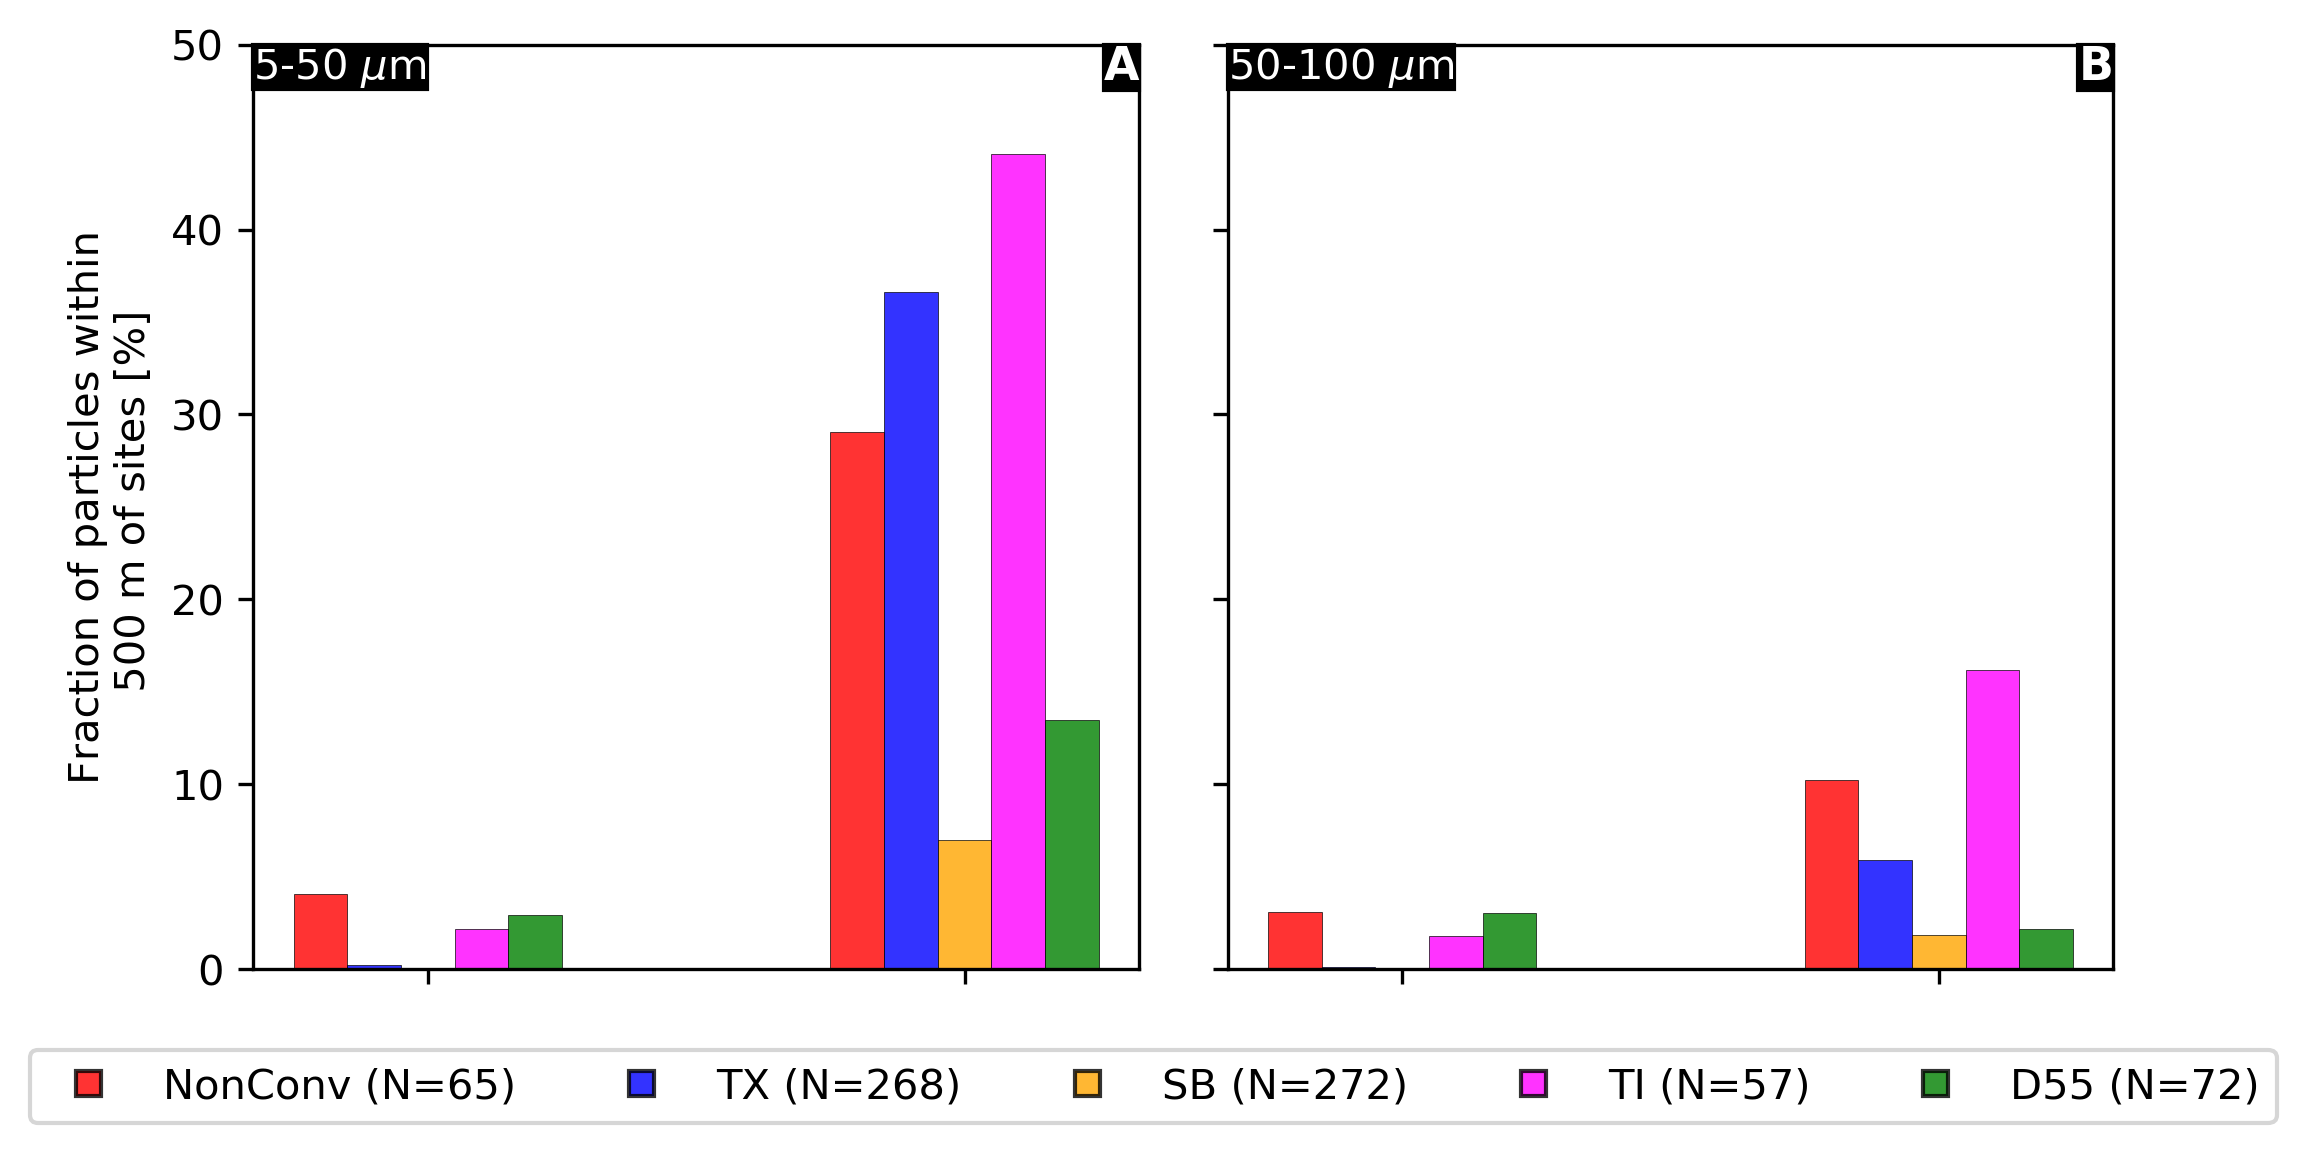
\includegraphics[width=\textwidth]{chapters/onset/figures/aggregated_new.png}
	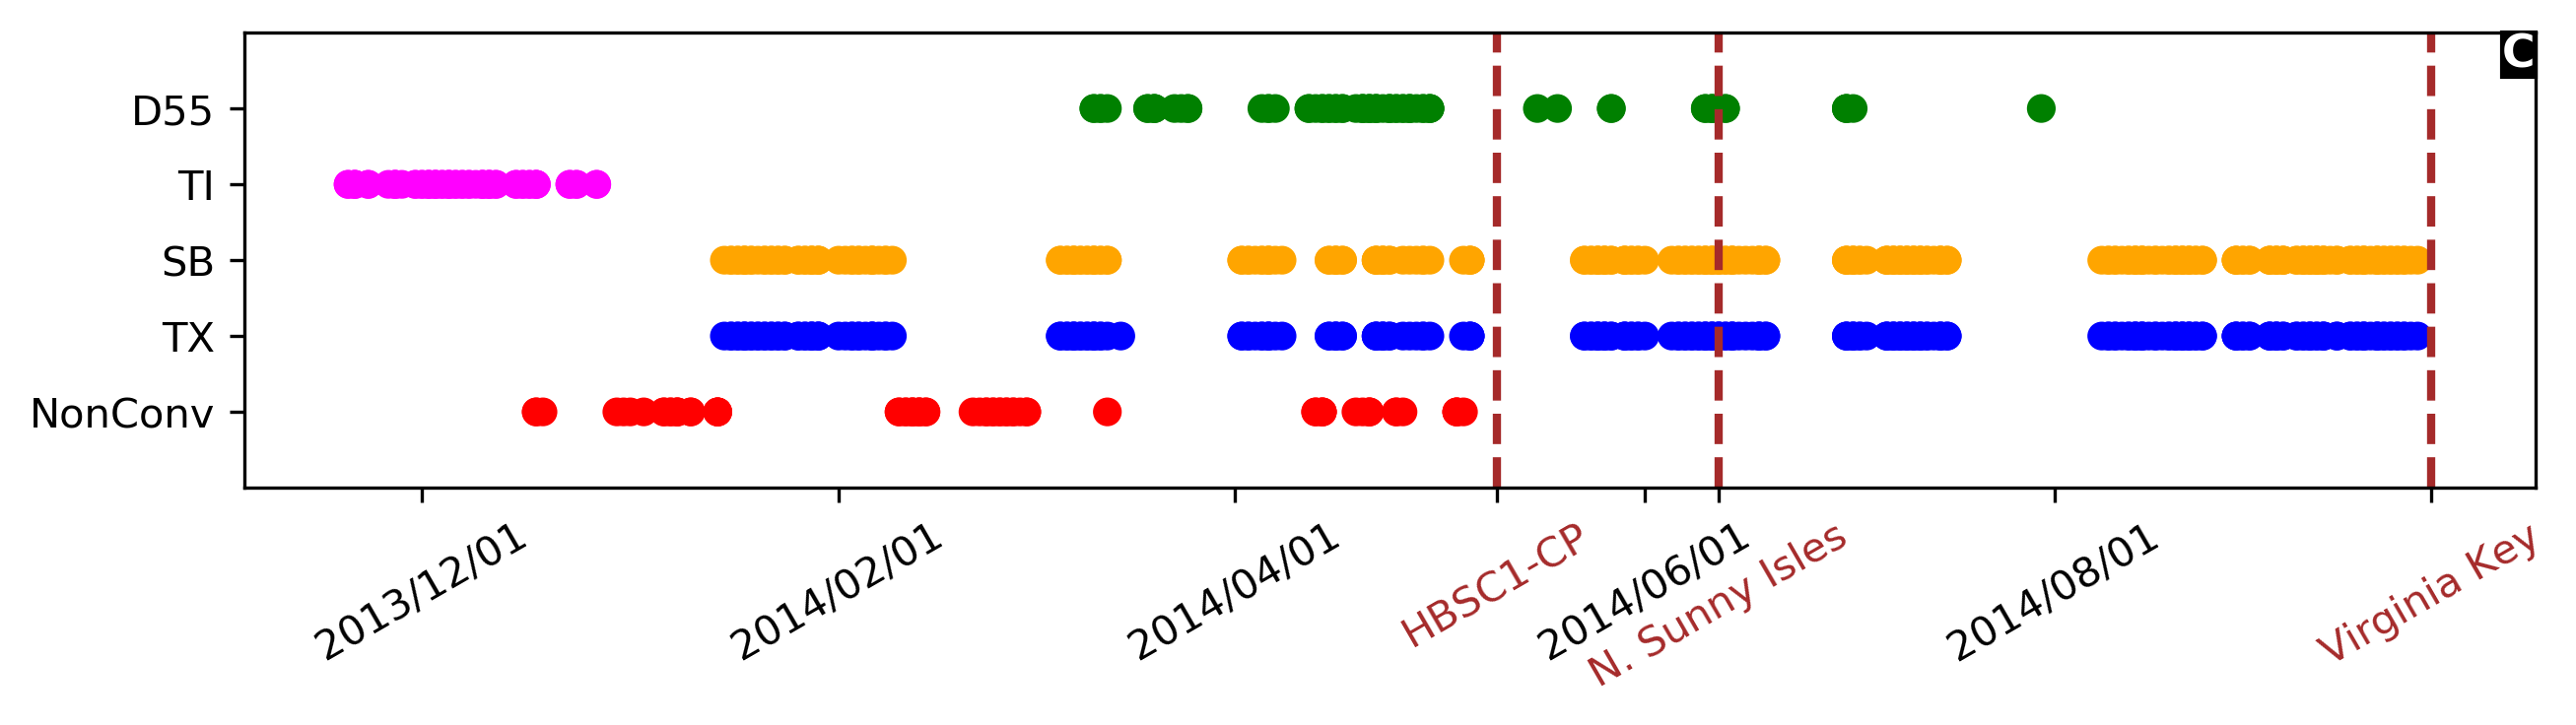
\includegraphics[width=\textwidth]{chapters/onset/figures/timeline.png}
	\caption{Fraction of the total number of sediment particles released by each type of dredge that drifted within 500 of HBSC1-CP and N. Sunnny Isles with grain sized of 5-50 $\mu$m (\textbf{A}) and 50-100 $\mu$m (\textbf{B}). \textbf{C}: Temporal distribution of the simulated dredging operations. The dates of the first reported disease signs at each monitoring site are shown with dotted vertical lines in dark red. With the exception of HBSC1-CP, sites located south to the dredged channel were barely impacted by the dredging. However, a significant fraction of the released sediment particles reached the northern site of N. Sunny Isles. The number of simulated dredging operations is given between brackets for each dredging type}
	\label{fig:onset_bar}
\end{figure}

Applying the same analysis to the discharge pipe of Miami Central District Municipal WWTP suggested that only wastewater released from a leak in the direct vicinity of the Virginia Key could have impacted the site. Fig. \ref{fig:onset_pipe} shows the fraction of released wastewater particles that reached the site of Virginia Key for every 100 m segments of the discharge pipe. The fraction of particles that drifted within 500 m of Virginia Key was: 100\% for particles released within 500 m of the site; 0-1\% for particles released between 500 m and 1.5 km away from the site; and 0\% for all other sources of wastewater particles. As HBSC1-CP was also located near the discharge pipe, a similar analysis was conducted for this monitoring site and gave similar results.

\begin{figure}
	\centering
	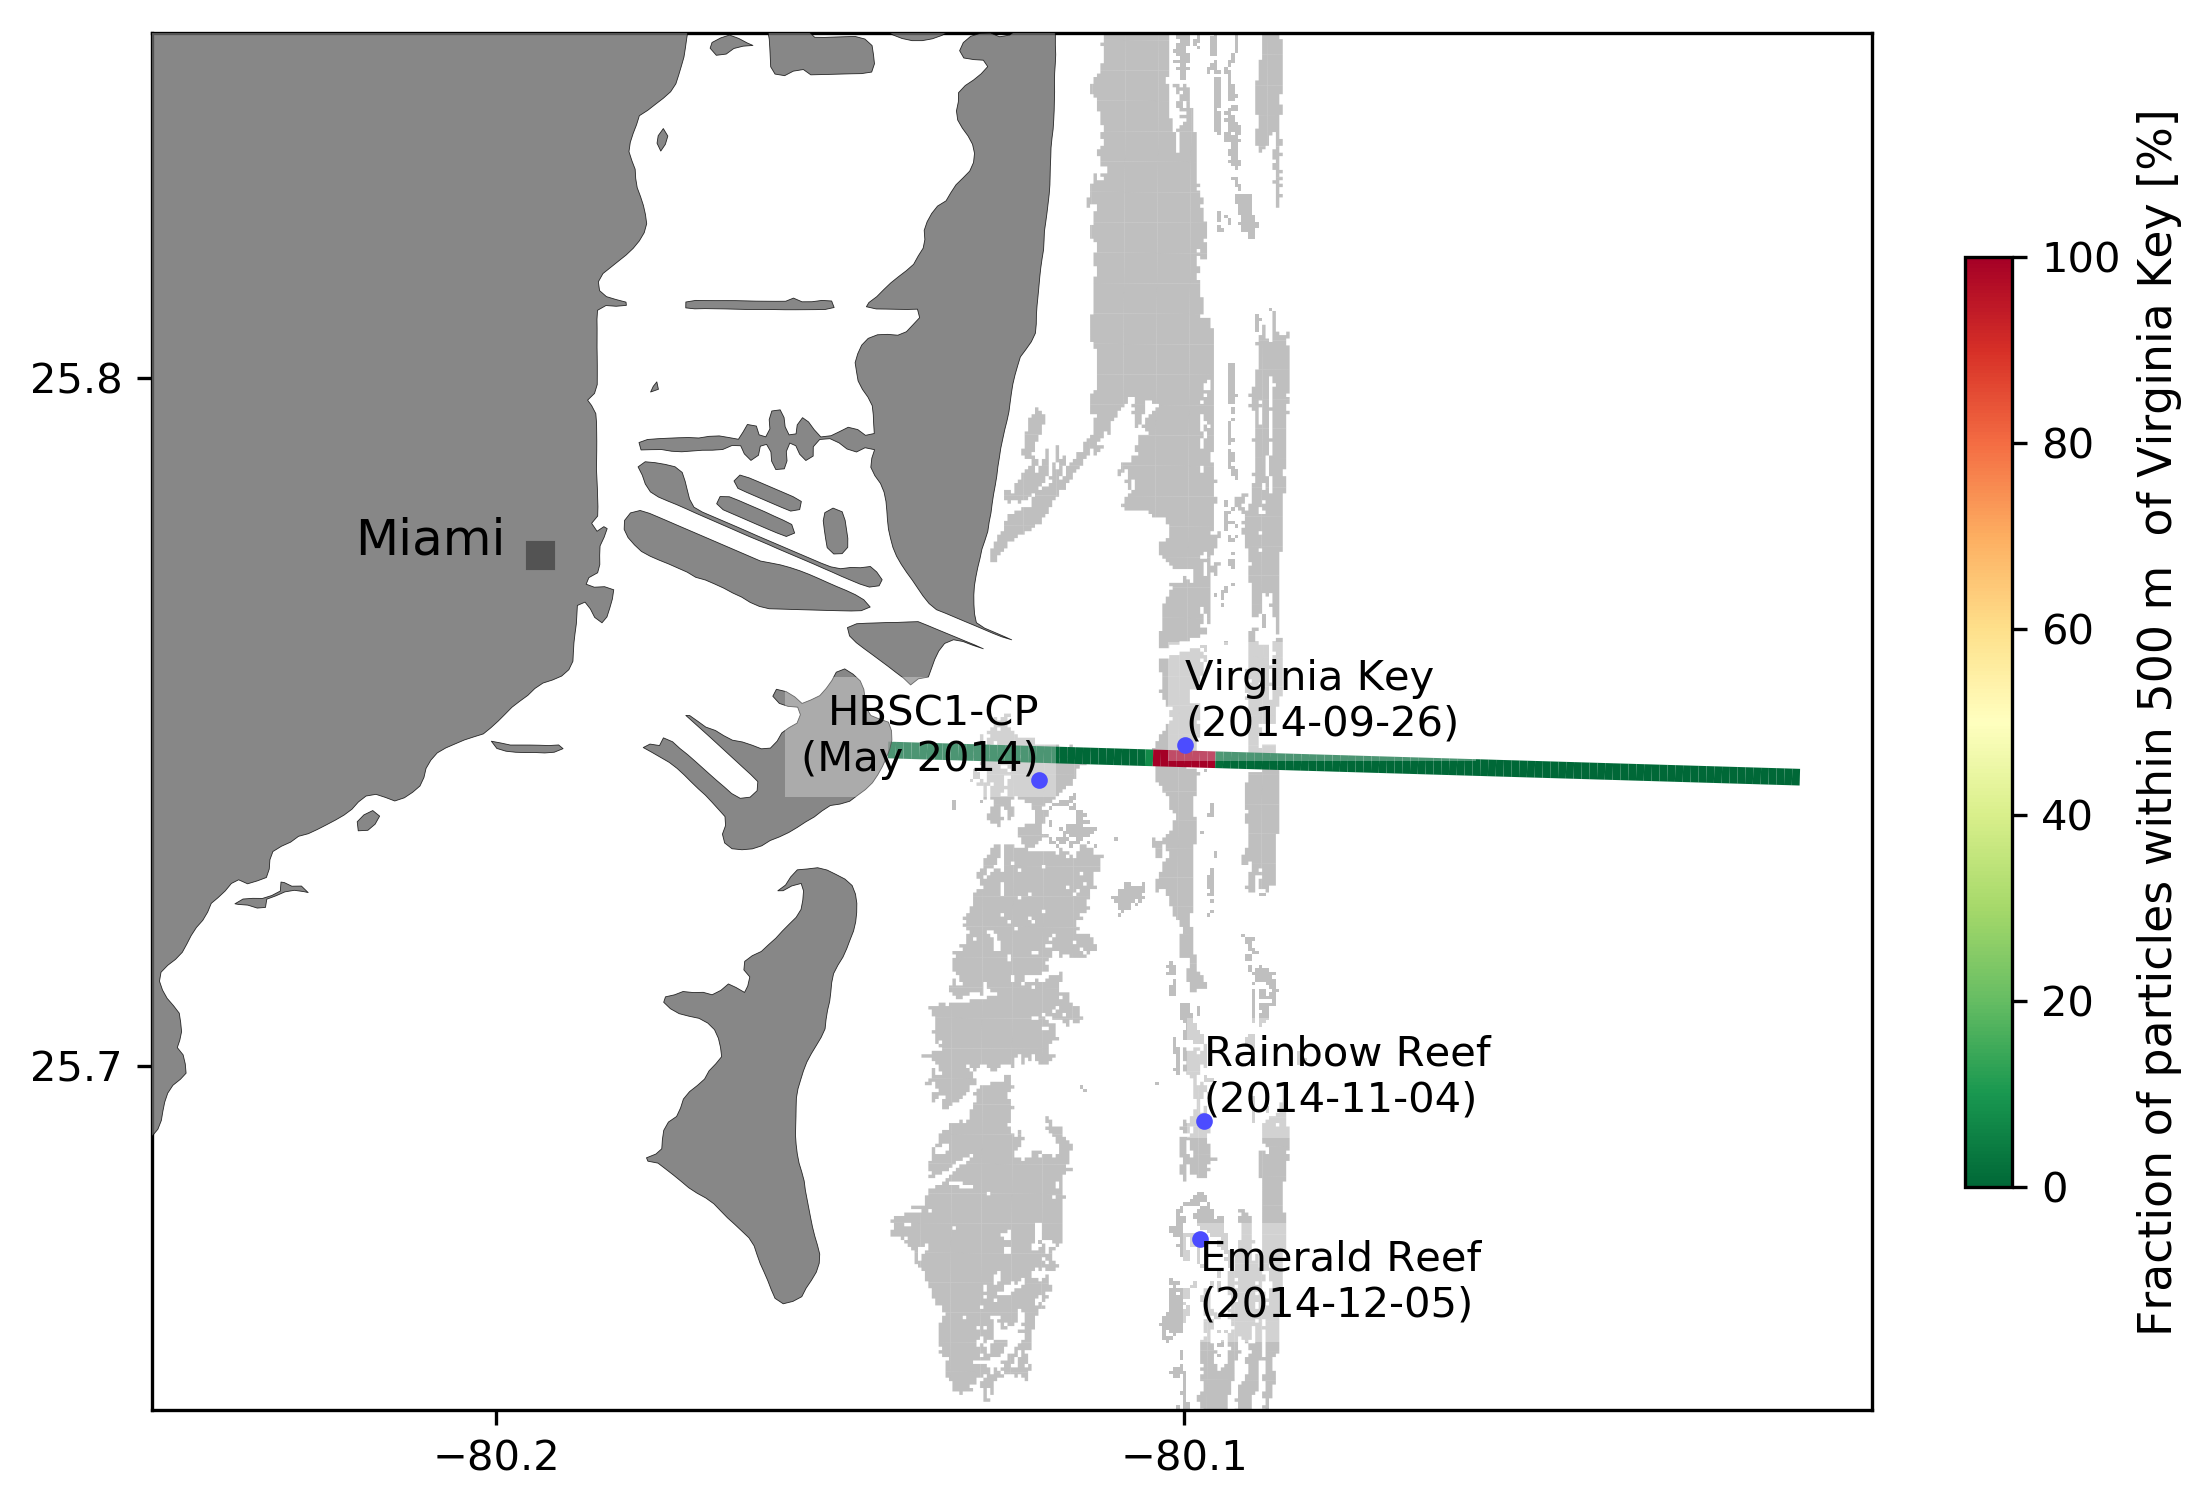
\includegraphics[width=.7\textwidth]{chapters/onset/figures/pipeline.png}
	\caption{Fraction of wastewater particles reaching the site of Virginia Key for potential leak positions located every 100 m along the discharge pipe. Only particles released in the direct vicinity of Virginia Key could reach the monitoring site.}
	\label{fig:onset_pipe}
\end{figure}

As signs of disease were observed at site HBSC1-CP in May 2014, before the first observations of SCTLD in Virginia Key in September 2014, we assessed the presence of shortest paths from HBSC1-CP to Virginia Key in the modeled monthly disease connectivity networks between May and September 2014 (Fig. \ref{fig:onset_path}). We found connectivity pathways connecting the two sites during all months of May-September 2014, with the exception of July. This suggests that there was a possibility of disease propagation from HBSC1-CP to Virginia Key during most of these 5 months. However, we found no direct pathway connecting the two sites. Southern intermediary reefs were systematically needed as stepping stones for the propagation of the disease. This suggests that several months might have been required for disease agents to reach Virginia Key from HBSC1-CP. Moreover, shortest paths in June, August and September 2014 had many sub-reef stepping stones in common. These similar connectivity patterns indicate favorable conditions for disease propagation over several months from HBSC1-CP to Virginia Key during this period.  

\begin{figure}
	\centering
	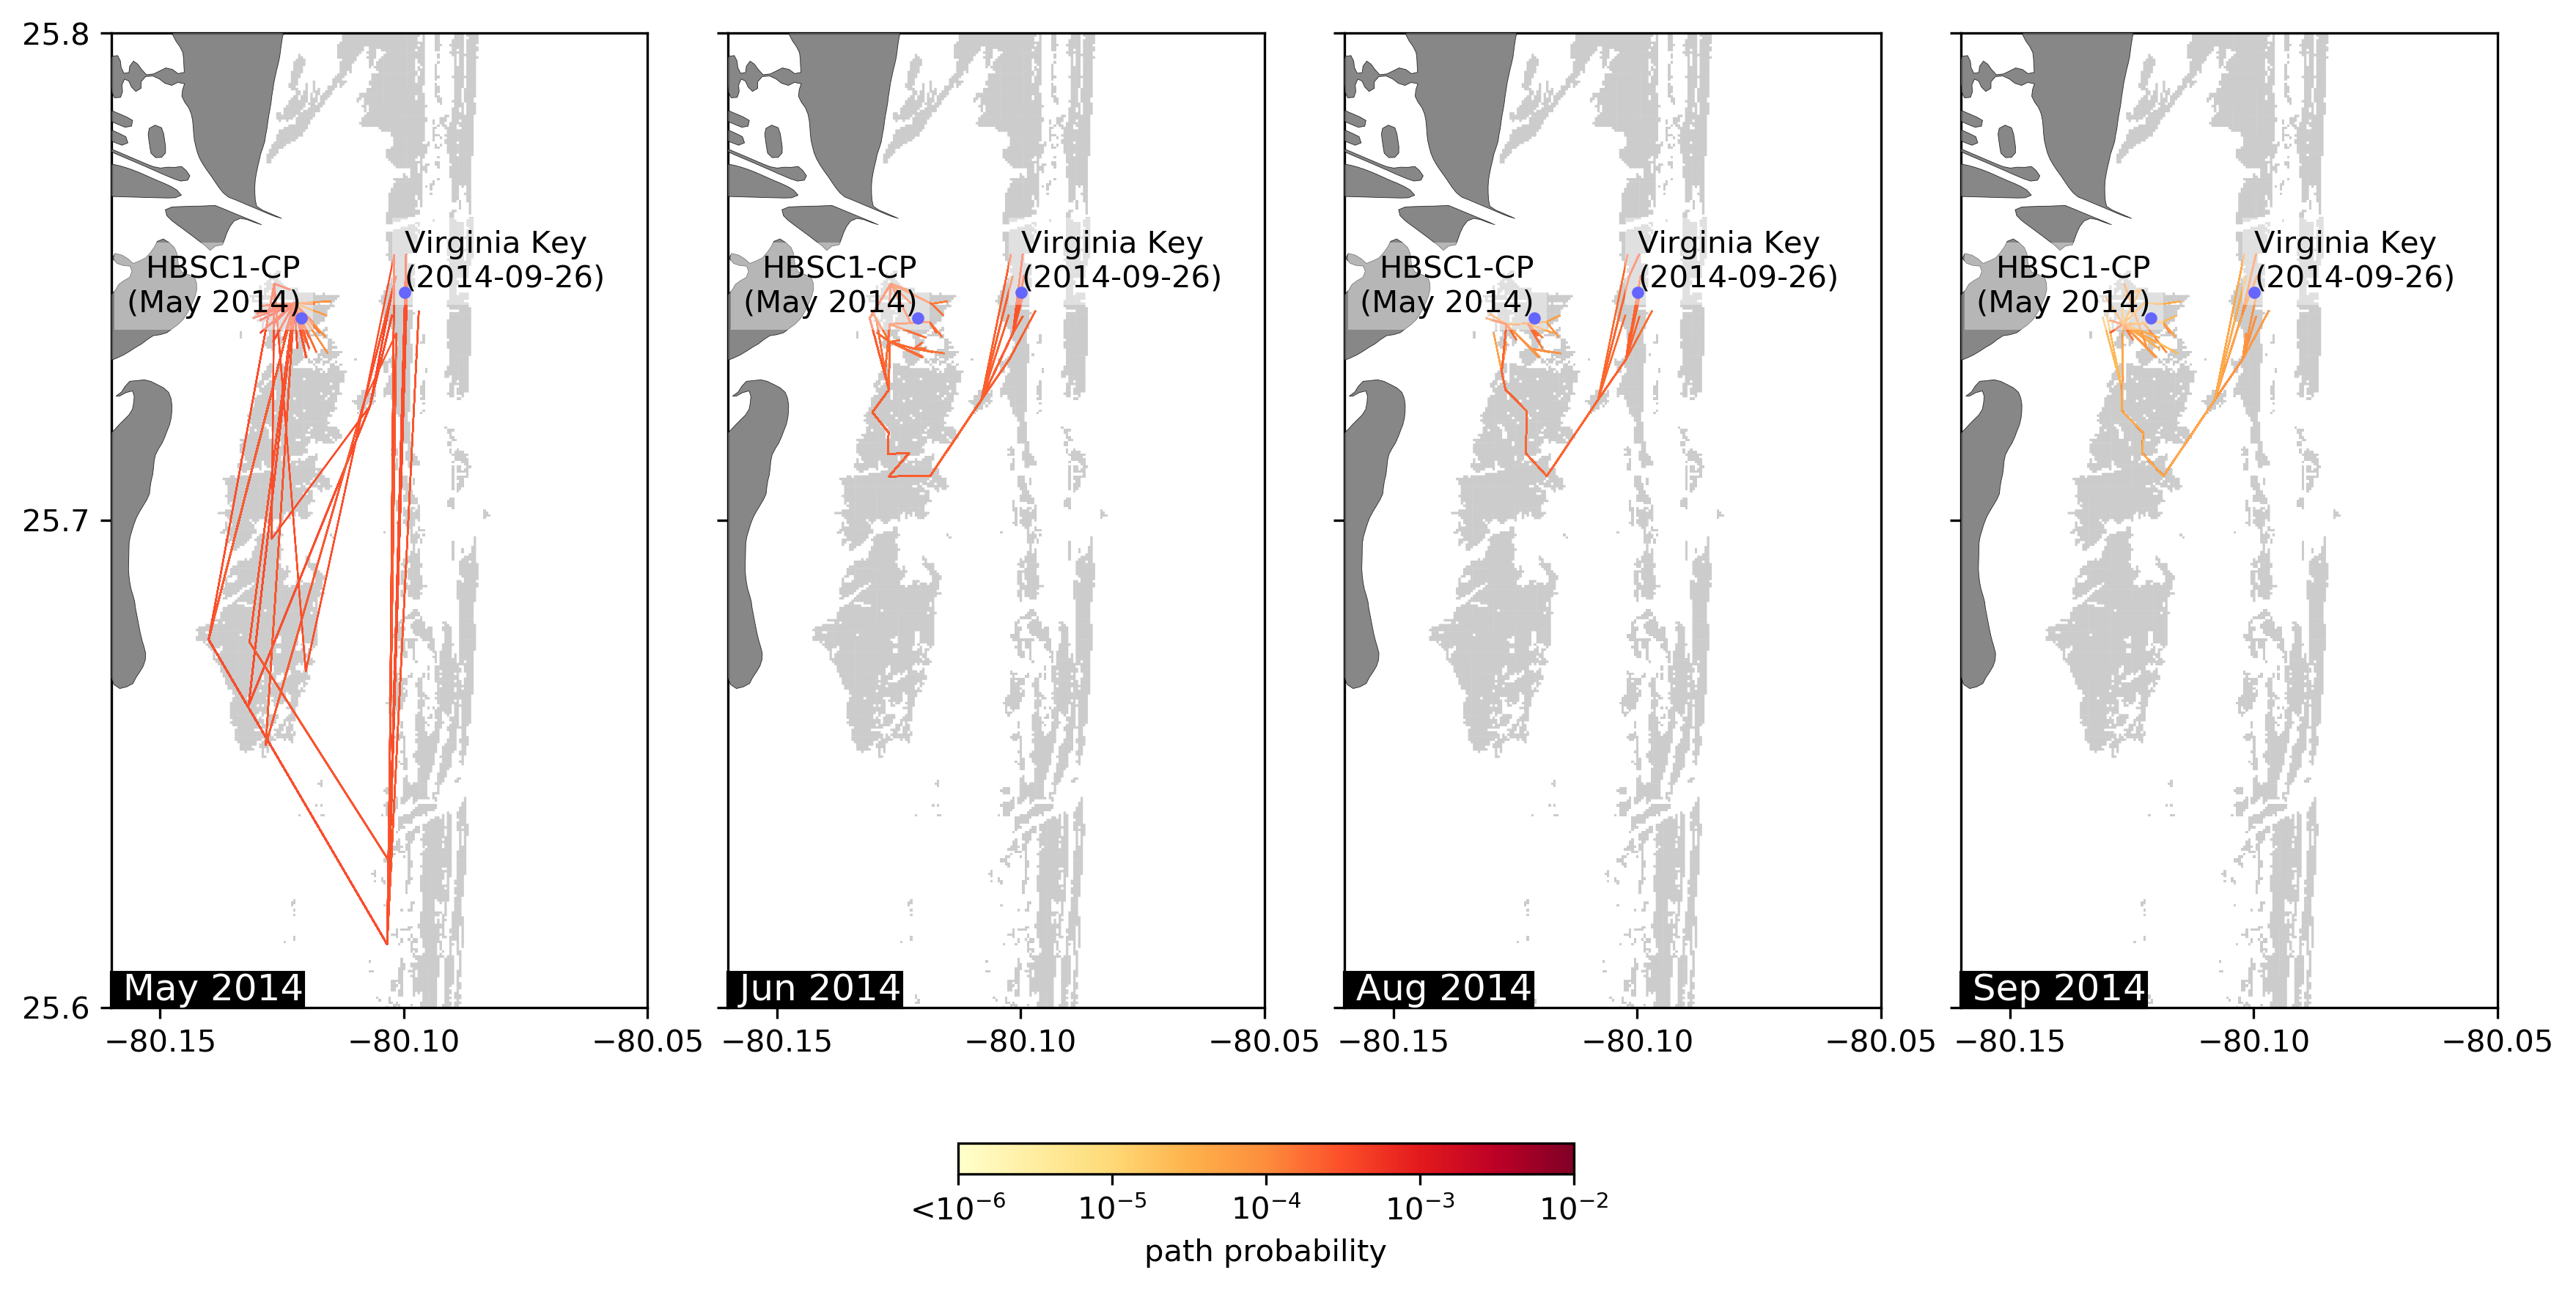
\includegraphics[width=\textwidth]{chapters/onset/figures/fig_paths.png}
	\caption{Shortest path from HBSC1-CP to Virginia Key in the monthly disease connectivity networks between May and September 2014. July 2014 was the only month without modeled connectivity between the two sites between May and September 2014. Southern intermediary reefs were needed as stepping stones for the propagation of the disease from HBSC1-CP to Virginia Key.}
	\label{fig:onset_path}
\end{figure}

% === DISCUSSION === %
\section{Discussion}

% SUMMARY
The quasi-3D sediment model forced by currents from the high-resolution coastal ocean model SLIM reproduced a sediment dynamics consistent with plume observations derived from satellite imagery. It suggests that sediment particles produced by dredging were mostly transported northward under the influence of the Florida Current. No sediment particles reached the southern sites of Rainbow Reef and Emerald Reef while dredging had limited direct impact on Virginia Key, identified as the site where the outbreak of SCTLD was initiated in September 2014 \citep{precht2016unprecedented}. Furthermore, our results indicate that it is unlikely that the site was affected by a leaking discharge pipe of Miami Central District Municipal WWTP, as suggested by \cite{gintert2019regional}. However, signs of disease were observed prior to September 2014 at the sites of N. Sunny Isles and HBSC1-CP, where the impact of dredging was greater. Up to 30\% of silt particles produced by non-conventional dredging operations reached coral reefs of N. Sunny Isles while 5\% of them reached site HBSC1-CP, where significant sedimentation occurred. Furthermore, monthly disease connectivity networks indicate that disease agents could be transmitted from HBSC1-CP to the site of Virginia Key.   

% LARGE IMPACT OF DREDGING
Our study confirms previous reports about the widespread impact of the expansion of PoM. As in \cite{barnes2015sediment}, the total area of plumes in our model was about 230 km$^2$. Furthermore, the model results reproduced the plume presence/absence within 15 km of the dredged channel derived by \cite{cunning2019extensive} with an accuracy of 82.7\%. Such a good agreement was only obtained for grain sizes in the range 5-50 $\mu$m, suggesting that fine silts were the main drivers of the turbidity generated by dredging, which is consistent with previous studies \citep{storlazzi2015influence,fourney2017additive}. Despite this good agreement, the distribution of plumes predicted by our model tends to be shifted northward compared to these previous studies. These discrepancies might be explained by the fact that our approaches is solely based on sediment concentration. However, turbidity depends on many local factors such as the water content of phytoplankton and organic matters \citep{gray2000comparability,thackston2000improved}. As reported by \cite{cunning2019extensive}, the plumes mostly occurred in areas of high sedimentation. As such areas were mostly located over coral reefs, our results suggests that the expansion of PoM might have harmed coral populations over an extended area through increased turbidity and sedimentation. This sedimentation mostly took place on alongshore reefs for grain sizes smaller than 50$\mu$m and on offshore reefs for coarser grain sizes. Sediment settlement might be significantly harmful to offshore coral reefs populations as they are usually less accustomed to sedimentation than their inshore  counterparts \citep{wolanski2005fine}.

% LIMITATION + SHOW THAT N. SUNNY ISLE AND HBSC1-CP WERE SIGNIFICANTLY IMPACTED
A limitation of our study is that conventional and non-conventional dredging are treated in the same way in the model. For all dredging types, sediment particles were released at the same rate in the model. Although conventional dredging was reported to release fine-grained sediments in the water column through dewatering and overflow from barges \citep{jones2016assessing}, the quantity of dredged material lost in the water was limited by the use of pumping mechanisms. In contrast, for non-conventional dredging, the suction mechanism was turned off, causing all chopped rock particles to be released in the water column. The numbers of particles reaching the monitoring sites were therefore likely underestimated for non conventional dredging operations. However, the fractions given in Fig. \ref{fig:onset_bar}A,B remain valid as they are relative to the total number of sediments released in the water column. The coral reefs of N. Sunny Isles appeared to be highly sensitive to fine-grained sediments produced by dredging (Fig. \ref{fig:onset_bar}). Furthermore, the non-conventional rock-chopping that took place between December 2013 and May 2014, was a non-negligible source of sediments to N. Sunny Isles, as up to 30\% of the released particles reached the site. As sediments have the potential to act as a SCTLD vector \citep{rosales2020rhodobacterales, studivan2022reef}, the dredging might therefore have contributed to the observed onset of the disease on the reefs of N. Sunny Isles in June 2014. Moreover, up to 5\% of the fined-grained sediments produced by non-conventional dredging reached the site HBSC1-CP before May 2014, when the disease was first reported there. Although this represents a more limited quantity of sediments, HBSC1 was within 2 km from the sites where non-conventional dredging took place, in a region where the model predicted an important sedimentation. Therefore, although fewer sediments reached HBSC1-CP, they had a higher probability to settle and to be in direct contact with corals. In addition to smothering corals and diverting their energy through sediment removal \citep{erftemeijer2012environmental}, these settled sediments are more likely to transmit the disease to the reefs.

% POSSIBILITY OF DISEASE PROPAGATION THROUGH WATERBORNE TRANSMISSION
In all simulations, the expansion of PoM had limited direct impact on Virginia Key, identified as the site where the outbreak was initiated in September 2014 \citep{precht2016unprecedented}. For all grain sizes, the fraction of sediment particles reaching Virginia Key remained below 1\%. It is therefore unlikely that sediments produced by the deepening of the channel brought the disease to the site. Furthermore, our simulation of leaking wastewater along the discharge pipe of Miami Central District Municipal WWTP suggests that currents were likely to flush wastewater away from Virginia Key. It was therefore unlikely that wastewater affected the site, except if the leak was located within hundreds of meters from the site. However, signs of disease were observed prior to September 2014 at the sites of N. Sunny Isles and HBSC1-CP, both of which were impacted by the dredging. Several studies showed evidence of waterborne transmission of SCTLD \citep{aeby2019pathogenesis,dobbelaere2020coupled,eaton2021measuring,meiling2021variable}. Disease agents might therefore have been transported by currents from one of the diseased sites to Virginia Key. As site HBSC-CP was the closest to Virginia Key, we built and analyzed monthly disease connectivity networks and found connectivity pathways from HBSC1 to Virginia Key in May, June, August and September 2014. This implied that the propagation of the disease from HBSC1-CP to Virginia Key through hydrodynamics-driven transport of disease agents was possible during these four months. All these pathways used reefs located further south as stepping stones. Therefore, the propagation of SCTLD to Virginia Key starting from HBSC1-CP required these intermediary reefs to be first infected by disease agents released from HBSC1-CP. Once diseased, these colonies would then send disease agents to affect the next colonies of the connectivity pathway until the outbreak reached Virginia Key. Assuming an averaged transmission time of the order of 5-10 days \citep{dobbelaere2020coupled}, disease propagation from HBSC1-CP to Virginia Key might have required several months. This is consistent with the 5-month period separating disease reports at these two sites. Moreover, the fact that June, August and September exhibited similar connectivity pathways suggests that disease propagation could indeed have occurred over several months without being interrupted by changing hydrodynamic conditions.

\section{Conclusion}

In the present study, we evaluated the impact of the dredging operations that took place during the deepening of the Port of Miami shipping channel on the neighboring coral reefs. This evaluation was performed using a quasi-3D sediment model forced by high-resolution currents from the coastal ocean model SLIM. As the first signs of SCTLD were reported during the PMDDP and since sediments may be a SCTLD vector, we aimed at answering two main questions. First, we wanted to evaluate the fraction of sediments produced by the PMDDP that reached Virginia Key and other monitoring sites where the disease was reported. Second, we evaluated the possibility of waterborne transmission of SCTLD to Virginia Key from other reefs impacted by the dredging. Doing so, we paid a special attention to the sediments produced by non conventional rock chopping during which pumping mechanisms were turned off, causing all chopped rock particles to be directly released in the water column.

Our results suggest that the dredging operations had close to no direct impact on the coral reefs of Virginia Key, indicating that disease transmission by sediments was extremely unlikely. However, our results show that the sediments released by the non conventional dredging operations had a non-negligible impact on the sites of N. Sunny Isles and HBSC1-CP, where signs of disease were observed before the outbreak was first reported at Virginia Key. This suggests that the sediments might have triggered the onset of the disease at these two sites. Furthermore, using a previously developed bio-physical model that successfully reproduced the observed spread of SCTLD, we show that there was a possibility of waterborne disease propagation from HBSC1-CP to Virginia Key.

This study suggests that the PMDDP might have played a role in the onset of the outbreak of SCTLD at Virginia Key, from where the disease was then reported to propagate through the entire FCR. Our work brings new insight on the impact of a major dredging project in Florida on the onset of one of the worst coral outbreaks on record in the Caribbean. It suggests that the potential to initiate a coral disease outbreak should be taken into account when considering future dredging projects.

\begin{subappendices}
	\section{Reported disease signs at site HBSC1-CP in May 2014}\label{onset:appendice}
	\begin{figure}
		\centering
		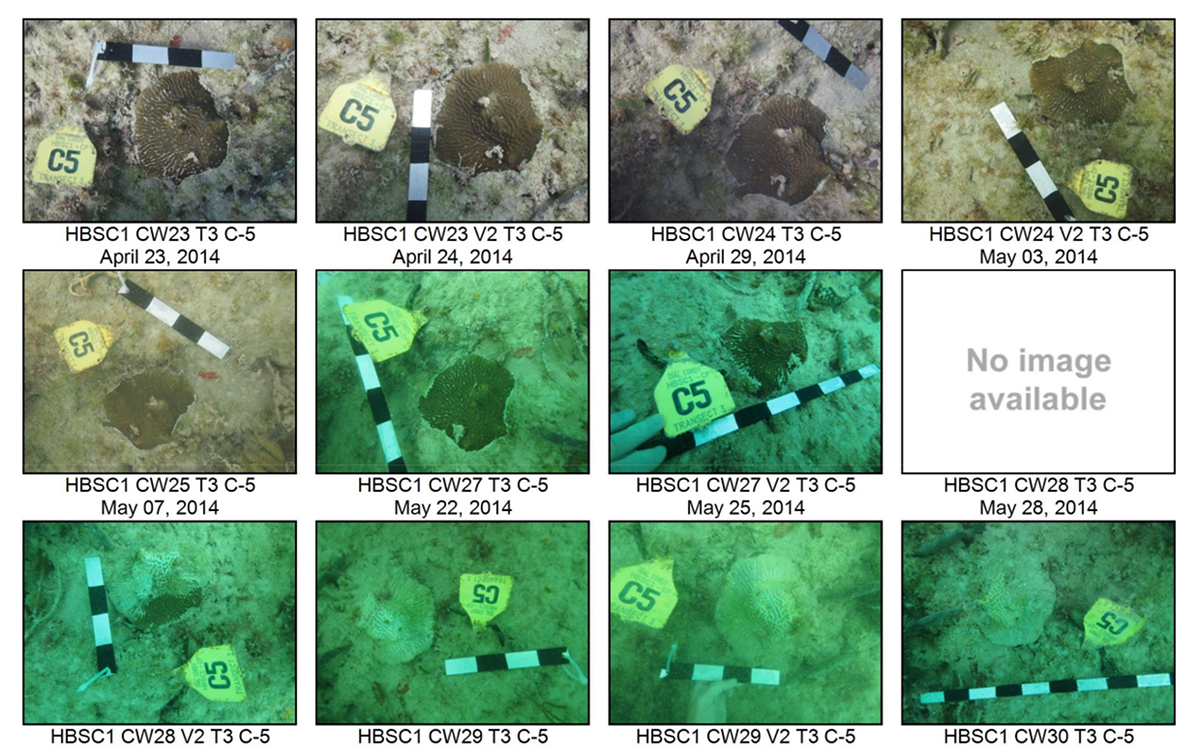
\includegraphics[width=\textwidth]{chapters/onset/figures/hbsc1_cp.png}
		\caption{Pictures of a monitored colony at site HBSC1-CP. The first signs of the disease appeared between May 25 and May 30. By June 4, the whole colony was completely dead}
	\end{figure}
\end{subappendices}